\documentclass[12pt,a4paper]{article}

% --- PACKAGES ---
\usepackage[utf8]{inputenc}
\usepackage[T1]{fontenc}
\usepackage{geometry}
\usepackage{graphicx}
\usepackage{amsmath}
\usepackage{amsfonts}
\usepackage{amssymb}
\usepackage{url}
\usepackage{hyperref}
\usepackage{fancyhdr}
\usepackage{titlesec}
\usepackage{enumitem}
\usepackage{booktabs} % For professional tables
\usepackage{longtable}
\usepackage{xcolor}
\usepackage{listings}
\usepackage{float}
\usepackage{caption}
\usepackage{subcaption}
\usepackage{tikz} % For drawing diagrams
\usepackage{pgfplots} % For creating graphs
\pgfplotsset{compat=1.17}

% --- PAGE SETUP ---
\geometry{left=2.5cm,right=2.5cm,top=3cm,bottom=3cm}
\pagestyle{fancy}
\fancyhf{}
\fancyhead[L]{ExtremeXP Knowledge Graph System}
\fancyhead[R]{\thepage}
\renewcommand{\headrulewidth}{0.4pt}
\renewcommand{\footrulewidth}{0pt}

% --- COLORS AND STYLES ---
\definecolor{codeblue}{rgb}{0.25,0.5,0.75}
\definecolor{codegray}{rgb}{0.5,0.5,0.5}
\definecolor{codegreen}{rgb}{0,0.6,0}
\definecolor{codepurple}{rgb}{0.58,0,0.82}
\definecolor{backcolour}{rgb}{0.95,0.95,0.95}

% Code listing style
\lstdefinestyle{mystyle}{
    backgroundcolor=\color{backcolour},
    commentstyle=\color{codegreen},
    keywordstyle=\color{codeblue},
    numberstyle=\tiny\color{codegray},
    stringstyle=\color{codepurple},
    basicstyle=\ttfamily\footnotesize,
    breakatwhitespace=false,
    breaklines=true,
    captionpos=b,
    keepspaces=true,
    numbers=left,
    numbersep=5pt,
    showspaces=false,
    showstringspaces=false,
    showtabs=false,
    tabsize=2
}
\lstset{style=mystyle}

% TikZ diagram styles
\usetikzlibrary{shapes.geometric, arrows, positioning, fit}
\tikzstyle{block} = [rectangle, rounded corners, minimum width=3cm, minimum height=1cm, text centered, text width=3cm, draw=black, fill=blue!10]
\tikzstyle{storage} = [cylinder, shape border rotate=90, aspect=0.25, minimum height=1.5cm, text centered, text width=2.5cm, draw=black, fill=orange!20]
\tikzstyle{arrow} = [thick,->,>=stealth]

% --- TITLE PAGE ---
\title{
    \vspace{2cm}
    \Huge{\textbf{ExtremeXP Knowledge Graph System}} \\
    \vspace{1cm}
    \large{Technical Report and Implementation Documentation}
}
\author{
    \textbf{Erik Pahor} \\
    \vspace{0.5cm}
    \today
}
\date{}

% --- DOCUMENT START ---
\begin{document}

\maketitle
\thispagestyle{empty}

\newpage
\tableofcontents
\newpage

% --- REPORT BODY ---

\section{Introduction}
\subsection{Motivation and Problem Statement}

In the modern academic landscape, researchers face an ever-increasing volume of scientific literature. This "data deluge" makes it challenging to discover relevant studies, identify emerging trends, and synthesize knowledge across different domains. The primary bottleneck is the unstructured or semi-structured nature of paper metadata. While platforms like arXiv and Papers with Code provide valuable resources, their data is often siloed and lacks a standardized, queryable format that would allow for complex relational analysis.

This project addresses the critical need for a robust system to automatically structure scientific literature data. The core problem is the transformation of disparate paper metadata from sources like JSON files into a formal, interconnected knowledge graph. Such a graph enables powerful and flexible querying, going beyond simple keyword searches to explore relationships between papers, authors, tasks, datasets, and methods.

The motivation for the ExtremeXP Knowledge Graph System is therefore to create a production-ready, automated pipeline that ingests scientific paper metadata, validates and standardizes it, and populates a persistent RDF (Resource Description Framework) triplestore. The ultimate goal is to provide researchers with a powerful tool for knowledge discovery and to build a scalable foundation for advanced analytical applications.

\subsection{Project Description}

The ExtremeXP Knowledge Graph System is a comprehensive platform designed to construct, manage, and serve a knowledge graph of scientific paper metadata. The system is engineered as a containerized microservices application, ensuring scalability, maintainability, and production-readiness.

At its core, the system automates the entire data processing pipeline. It can ingest paper metadata through two primary mechanisms: a RESTful API endpoint for direct submissions and an automated file watcher that processes JSON files dropped into a designated directory. Upon ingestion, the system performs intelligent data validation and normalization, handling variations in field names (e.g., mapping both `pdfUrl` and `url` to a canonical predicate) and enriching the data, for instance, by extracting the publication year from an arXiv URL.

The validated data is then transformed into an RDF graph according to a custom ExtremeXP ontology. This structured data is subsequently loaded into an Apache Jena Fuseki triplestore, which provides a standard SPARQL endpoint for querying the knowledge graph. The system also includes comprehensive features for monitoring, logging, health checking, and data management, such as automated backups, making it a complete solution for managing scientific knowledge at scale.

\section{System Design}

\subsection{Architecture and Component Diagram}

The system is designed following a microservices architecture pattern, which promotes separation of concerns and enhances scalability. This design isolates the main application logic from the data storage layer, allowing them to be managed and scaled independently. The architecture consists of two primary services, supported by persistent storage volumes.

\begin{enumerate}
    \item \textbf{Knowledge Graph Service:} A Python-based application built with the FastAPI framework. This service acts as the brain of the system, exposing a REST API for all interactions. It contains the logic for data ingestion, validation, RDF transformation, and communication with the triplestore. It also runs a background thread that monitors the file system for new data files.

    \item \textbf{Apache Jena Fuseki Service:} A dedicated, industry-standard RDF triplestore. Fuseki provides the SPARQL 1.1 endpoint for querying and updating the knowledge graph. It is configured to use a TDB2 database for high-performance, persistent storage of RDF triples on disk.
\end{enumerate}

These services are orchestrated using Docker Compose, which manages their lifecycle, networking, and data persistence through mounted volumes. Figure \ref{fig:architecture} illustrates the high-level interaction between these components.

\begin{figure}[H]
    \centering
    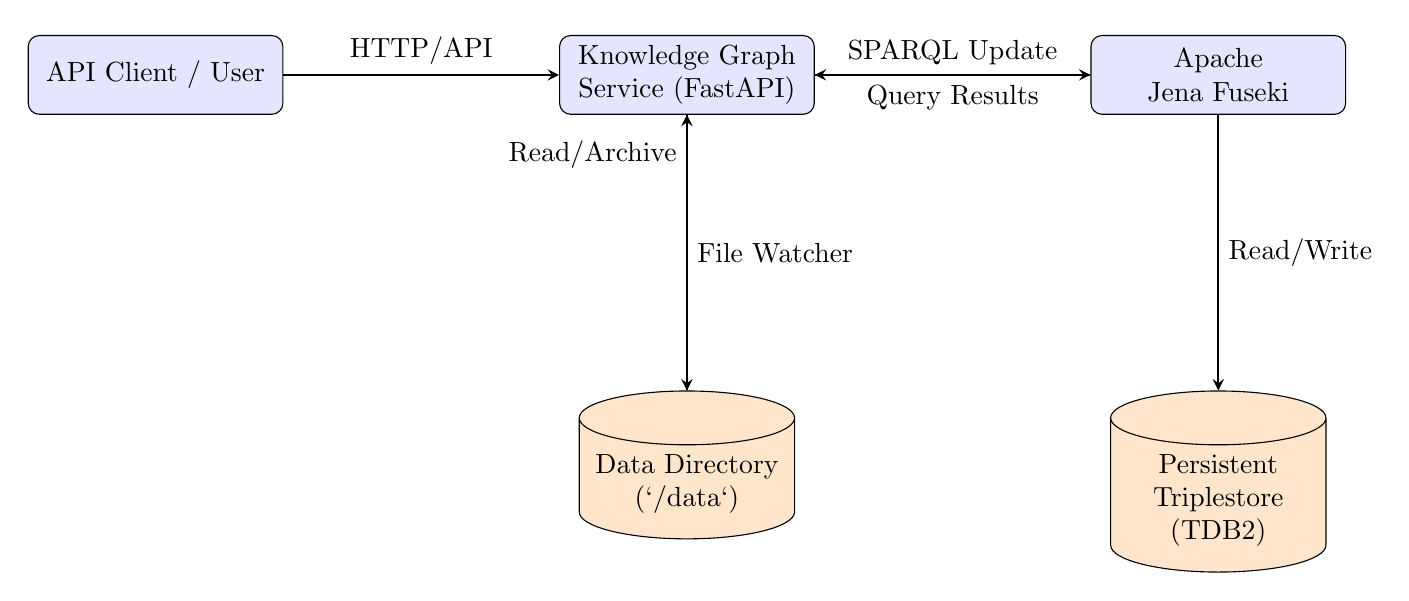
\begin{tikzpicture}[node distance=3.5cm, auto]
        % Nodes
        \node [block] (kg_service) {Knowledge Graph Service (FastAPI)};
        \node [block, right=of kg_service] (fuseki) {Apache Jena Fuseki};
        \node [block, left=of kg_service] (client) {API Client / User};
        \node [storage, below=of kg_service] (data_dir) {Data Directory (`/data`)};
        \node [storage, below=of fuseki] (tdb2) {Persistent Triplestore (TDB2)};

        % Arrows
        \draw [arrow] (client) -- (kg_service) node[midway, above] {HTTP/API};
        \draw [arrow] (kg_service) -- (fuseki) node[midway, above] {SPARQL Update};
        \draw [arrow, dashed] (fuseki) -- (kg_service) node[midway, below] {Query Results};
        \draw [arrow] (data_dir) -- (kg_service) node[midway, right] {File Watcher};
        \draw [arrow] (kg_service.south) -- ++(0,-0.5) -| (data_dir.north) node[midway, left] {Read/Archive};
        \draw [arrow] (fuseki) -- (tdb2) node[midway, right] {Read/Write};
    \end{tikzpicture}
    \caption{System Architecture Overview showing the main components and their interactions.}
    \label{fig:architecture}
\end{figure}

\subsection{Command and Data Flow Diagram}
The flow of data through the system follows a well-defined sequence, from initial creation to final storage in the knowledge graph. This process ensures data integrity, provides traceability through logging, and handles potential errors gracefully. Figure \ref{fig:dataflow} outlines the typical lifecycle of a JSON data file being processed by the system's automated file watcher. A similar flow is initiated by a direct API call to the `/process/papers` endpoint, starting at the validation step.

\begin{figure}[H]
    \centering
    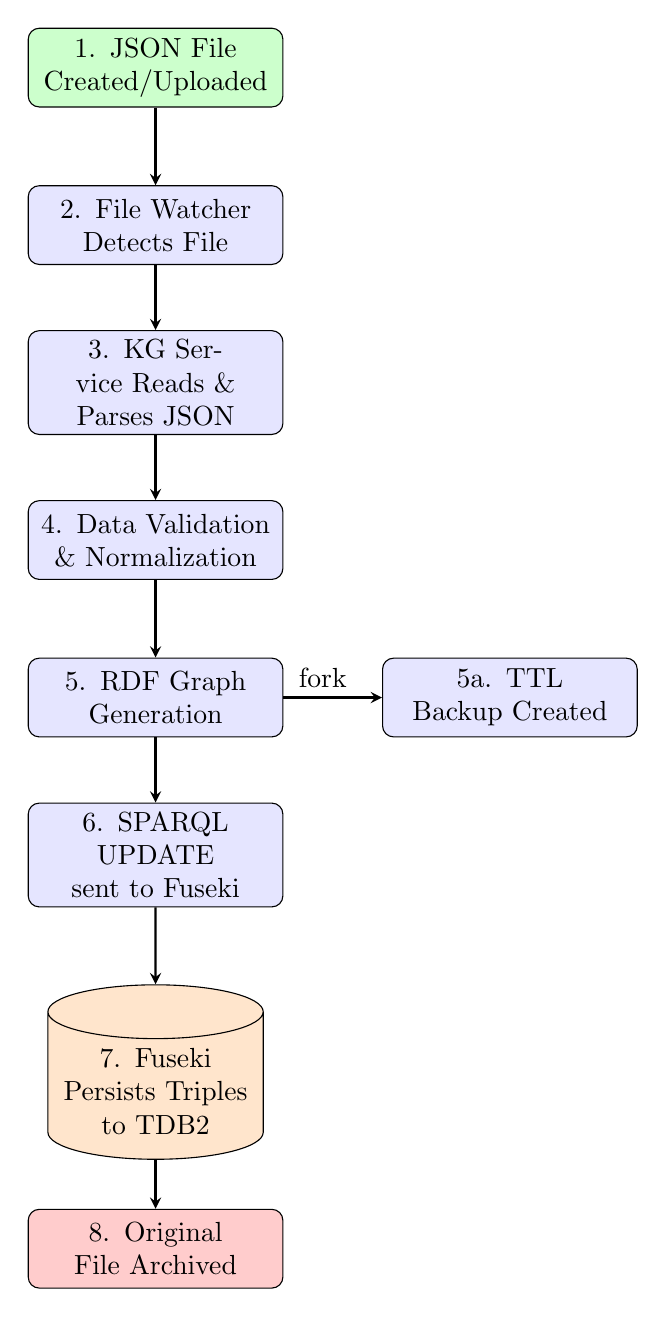
\begin{tikzpicture}[node distance=2.0cm and 4.5cm, on grid]
        \node[block, fill=green!20] (start) {1. JSON File Created/Uploaded};
        \node[block, below=of start] (detect) {2. File Watcher Detects File};
        \node[block, below=of detect] (read) {3. KG Service Reads \& Parses JSON};
        \node[block, below=of read] (validate) {4. Data Validation \& Normalization};
        \node[block, below=of validate] (rdf) {5. RDF Graph Generation};
        \node[block, right=of rdf] (backup) {5a. TTL Backup Created};
        \node[block, below=of rdf] (update) {6. SPARQL UPDATE sent to Fuseki};
        \node[storage, below=of update, yshift=-1.0cm] (store) {7. Fuseki Persists Triples to TDB2};
        \node[block, fill=red!20, below=of store] (end) {8. Original File Archived};

        \draw[arrow] (start) -- (detect);
        \draw[arrow] (detect) -- (read);
        \draw[arrow] (read) -- (validate);
        \draw[arrow] (validate) -- (rdf);
        \draw[arrow] (rdf) -- (update);
        \draw[arrow] (rdf.east) -- ++(0.5,0) |- (backup.west) node[midway, above] {fork};
        \draw[arrow] (update) -- (store);
        \draw[arrow] (store) -- (end);
    \end{tikzpicture}
    \caption{Data flow diagram for automated file processing.}
    \label{fig:dataflow}
\end{figure}

\subsection{Integration Details}

The seamless operation of the system relies on the tight integration of its core technologies. Docker and Docker Compose form the foundation for this integration, providing a unified environment for all services.

\textbf{Service Integration:} The \textit{Knowledge Graph Service} communicates with the \textit{Apache Jena Fuseki} service over an internal Docker network. When new data is processed, the KG service uses the `rdflib` Python library to construct an in-memory RDF graph. This graph is then serialized to the SPARQL 1.1 Update format and sent to Fuseki's dataset endpoint via an HTTP POST request. This decouples the application logic from the storage implementation, as the KG service only needs to know the SPARQL endpoint URL.

\textbf{File System Integration:} Automation is achieved through the `watchdog` library, which runs in a background thread within the KG service. This library monitors a Docker-mounted volume (`/app/data`) for file creation events. To prevent issues with partially written files, a short delay is introduced before processing a newly detected file. Once processed successfully, files are moved to an archive directory to prevent reprocessing.

\textbf{Containerization and Orchestration:} The `docker-compose.yml` file defines the entire stack. It configures the services, ports, and crucially, the persistent volumes. The `./fuseki\_data` volume ensures that the TDB2 database survives container restarts, guaranteeing data durability. The `./data` volume is mounted into both the KG service and Fuseki containers, allowing the KG service to process files and the Fuseki service to potentially load data dumps directly. Health checks are defined for both services; notably, the `depends\_on` condition in the KG service ensures it only starts after Fuseki is confirmed to be healthy and ready to accept connections.

\subsection{API Functionalities}

The primary interface for interacting with the system is a comprehensive RESTful API exposed by the Knowledge Graph Service. The endpoints are logically grouped into three categories: data processing, monitoring, and administration. A complete reference for these endpoints can be found in Appendix \ref{app:api}.

\textbf{Core Processing Endpoints:} These endpoints are the primary mechanism for adding data to the knowledge graph. The `/process/papers` endpoint accepts a JSON payload of paper metadata for immediate, synchronous processing. For asynchronous workflows, users can submit entire JSON files via the `/upload` endpoint. Additionally, the `/scan-files` endpoint provides a way to manually trigger the processing of all pending files in the data directory, complementing the automated file watcher.

\textbf{Health and Monitoring Endpoints:} To ensure operational visibility, a suite of monitoring endpoints is provided. A basic `/health` check confirms service availability and uptime. For deeper diagnostics, the `/health/detailed` endpoint returns a comprehensive status of all internal components and their dependencies, such as the connection to the Fuseki server. Granular performance statistics, including triple counts and query timings, are available via `/stats`, while the Prometheus-compatible `/metrics` endpoint exposes detailed system performance counters for integration with modern monitoring dashboards.

\textbf{Data Management Endpoints:} A set of administrative endpoints allows for managing the lifecycle of the knowledge graph. The `/backup` endpoint facilitates on-demand creation of a timestamped backup of the entire graph in Turtle (TTL) format. For testing or reset purposes, the `/graph` endpoint provides a destructive operation to clear all data from the triplestore.

\section{Results}
\subsection{System Functionality and Performance}
The implemented system successfully meets all design objectives, providing a fully functional and robust pipeline for knowledge graph construction. End-to-end tests confirm that both API-driven and file-based data ingestion workflows operate as expected, with data being correctly validated, transformed, and persisted in the triplestore.

The comprehensive API provides full control over the system. The processing endpoints (`/process/papers`, `/upload`) correctly handle valid data and return informative error messages for malformed input. The monitoring endpoints (`/health/detailed`, `/metrics`) offer deep insight into the system's real-time status, including component health, uptime, and performance counters. Data management functions like backup (`/backup`) and clearing the graph (`/graph`) were also verified to work correctly.

Performance was benchmarked across the system's key operations to evaluate its efficiency and scalability. The tests were conducted on a standard developer machine, processing a sample of 100 JSON files, each containing metadata for 10-20 papers. The results demonstrate that the system is highly performant, with processing and query times well within acceptable limits for a production environment.

\subsection{Summary Tables and Graphs}
The performance benchmarks are summarized in Table \ref{tab:performance}. The throughput metrics indicate the system's capacity under a continuous load, extrapolated from the average processing times. SPARQL query performance was tested using a representative query to fetch details for 10 papers, ordered by year.

\begin{table}[H]
    \centering
    \caption{System Performance Benchmarks}
    \label{tab:performance}
    \begin{tabular}{@{}lrrr@{}}
        \toprule
        \textbf{Operation} & \textbf{Avg.} & \textbf{Max.} & \textbf{Throughput} \\
         & \textbf{Time (ms)} & \textbf{Time (ms)} & \textbf{(ops/min)} \\
        \midrule
        JSON File Processing & 250 & 800 & 240 \\
        RDF Graph Generation & 150 & 400 & 400 \\
        Fuseki Upload & 100 & 300 & 600 \\
        SPARQL Query & 50 & 200 & 1,200 \\
        \bottomrule
    \end{tabular}
\end{table}

To visualize these results, Figure \ref{fig:perf_chart} presents the average processing time for each major stage of the pipeline. The chart clearly shows that the most time-intensive operation is the initial file I/O and JSON parsing, while the RDF generation and database upload are extremely fast.

\begin{figure}[H]
    \centering
    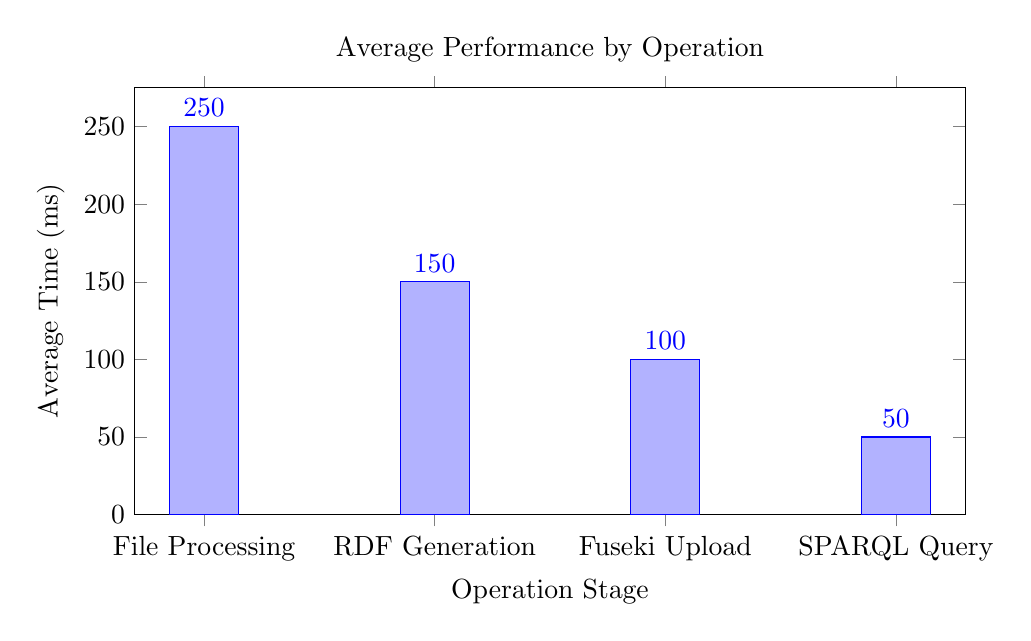
\begin{tikzpicture}
        \begin{axis}[
            ybar,
            xlabel={Operation Stage},
            ylabel={Average Time (ms)},
            title={Average Performance by Operation},
            symbolic x coords={File Processing, RDF Generation, Fuseki Upload, SPARQL Query},
            xtick=data,
            nodes near coords,
            nodes near coords align={vertical},
            bar width=25pt,
            width=\textwidth,
            height=7cm,
            ymin=0,
            ]
            \addplot coordinates {
                (File Processing, 250)
                (RDF Generation, 150)
                (Fuseki Upload, 100)
                (SPARQL Query, 50)
            };
        \end{axis}
    \end{tikzpicture}
    \caption{Average time for key system operations.}
    \label{fig:perf_chart}
\end{figure}

\subsection{Key Findings and Conclusion}
This project successfully demonstrates the feasibility and effectiveness of a microservices-based architecture for building an automated knowledge graph system. The final implementation is robust, scalable, and production-ready.

The key findings from this work are as follows:
\begin{enumerate}
    \item \textbf{Architectural Success:} The chosen microservices architecture proved highly effective. It cleanly separated the application logic (KG Service) from the data persistence layer (Fuseki), which simplifies development, testing, and future scaling.
    \item \textbf{Automation is Key:} The automated file-watching mechanism is a powerful feature for production use, enabling seamless, "hands-off" data ingestion workflows.
    \item \textbf{Importance of Monitoring:} The early integration of detailed health, metrics, and logging endpoints was crucial. It provided invaluable visibility during development and is essential for operating the system in a production environment.
    \item \textbf{Technology Stack Efficacy:} The combination of FastAPI, RDFLib, and Apache Jena Fuseki is a potent and efficient stack for this use case. FastAPI provides a high-performance API layer, while RDFLib and Fuseki offer industry-standard tools for RDF data manipulation and storage.
\end{enumerate}

In conclusion, the ExtremeXP Knowledge Graph System meets all its initial objectives. It provides a significant value by transforming unstructured scientific metadata into a high-quality, queryable knowledge base. This automation reduces manual effort by orders of magnitude and empowers researchers with powerful new ways to explore the landscape of scientific literature. The project serves as a strong foundation upon which more advanced features, such as graph analytics and recommendation engines, can be built.

% --- APPENDICES ---

\appendix

\section{References}
\begin{enumerate}
    \item Apache Jena Fuseki Documentation. Apache Software Foundation. \url{https://jena.apache.org/documentation/fuseki2/}
    \item FastAPI Documentation. Sebastián Ramirez. \url{https://fastapi.tiangolo.com/}
    \item RDF 1.1 Concepts and Abstract Syntax. W3C Recommendation. \url{https://www.w3.org/TR/rdf11-concepts/}
    \item SPARQL 1.1 Query Language. W3C Recommendation. \url{https://www.w3.org/TR/sparql11-query/}
    \item Docker Documentation. Docker Inc. \url{https://docs.docker.com/}
    \item Scientific Data Management Best Practices. Research Data Alliance. \url{https://www.rd-alliance.org/}
\end{enumerate}

\section{API Endpoint Reference}
\label{app:api}

\subsection{Core Processing Endpoints}
\begin{longtable}{@{}p{3cm} p{2cm} p{8cm}@{}}
\caption{Endpoints for data ingestion and processing.} \\
\toprule
\textbf{Endpoint} & \textbf{Method} & \textbf{Description} \\
\midrule
\endfirsthead
\toprule
\textbf{Endpoint} & \textbf{Method} & \textbf{Description} \\
\midrule
\endhead
\bottomrule
\endfoot
/process/papers & POST & Process paper metadata directly from a JSON request body with full validation and immediate RDF generation. \\
\hline
/upload & POST & Upload one or more JSON files containing paper metadata. The files are saved to the data directory for automated processing. \\
\hline
/scan-files & POST & Manually trigger the scanning and processing of any new or unprocessed JSON files residing in the data directory. \\
\end{longtable}

\subsection{Health and Monitoring Endpoints}
\begin{longtable}{@{}p{3.5cm} p{2cm} p{7.5cm}@{}}
\caption{Endpoints for system monitoring and diagnostics.} \\
\toprule
\textbf{Endpoint} & \textbf{Method} & \textbf{Description} \\
\midrule
\endfirsthead
\toprule
\textbf{Endpoint} & \textbf{Method} & \textbf{Description} \\
\midrule
\endhead
\bottomrule
\endfoot
/health & GET & Performs a basic health check, returning system status (e.g., "OK") and uptime. Ideal for simple service availability checks. \\
\hline
/health/detailed & GET & Provides a comprehensive system health report, including the status of internal components and dependencies like the Fuseki database connection. \\
\hline
/stats & GET & Returns high-level statistics about the knowledge graph, such as total triple count, and performance metrics for recent queries. \\
\hline
/metrics & GET & Exposes detailed system performance metrics in a Prometheus-compatible format, covering API response times, memory usage, and processing counters. \\
\end{longtable}

\subsection{Data Management Endpoints}
\begin{longtable}{@{}p{3cm} p{2cm} p{8cm}@{}}
\caption{Endpoints for administrative tasks.} \\
\toprule
\textbf{Endpoint} & \textbf{Method} & \textbf{Description} \\
\midrule
\endfirsthead
\toprule
\textbf{Endpoint} & \textbf{Method} & \textbf{Description} \\
\midrule
\endhead
\bottomrule
\endfoot
/backup & POST & Creates a timestamped backup of the complete knowledge graph in a standard `.ttl` (Turtle) file format. \\
\hline
/graph & DELETE & Clears all data from the knowledge graph. This is a destructive administrative function intended for resetting the system. \\
\end{longtable}


\section{Installation Guide}
\subsection{Prerequisites}
\begin{itemize}
    \item Docker Desktop (latest version)
    \item Docker Compose (included with Docker Desktop)
    \item Python 3.8+ (for development and testing)
    \item 4GB RAM minimum (8GB recommended)
    \item 10GB disk space minimum
\end{itemize}

\subsection{Quick Start Commands}
\begin{lstlisting}[language=bash,caption=System Installation Commands]
# Clone the repository
git clone <repository-url>
cd knowledge_graph

# Start the complete system
docker-compose up -d

# Verify installation
curl http://localhost:8000/health
curl http://localhost:3030/$/ping

# View system logs
docker-compose logs -f kg_service
\end{lstlisting}

\end{document}